%%% LaTeX Template
%%% This template can be used for both articles and reports.
%%%
%%% Copyright: http://www.howtotex.com/
%%% Date: February 2011

%%% Preamble
\documentclass[paper=a4, fontsize=11pt]{scrartcl}	% Article class of KOMA-script with 11pt font and a4 format
\usepackage[margin=0.7in]{geometry}
\usepackage[english]{babel}															% English language/hyphenation
\usepackage[protrusion=true,expansion=true]{microtype}				% Better typography
\usepackage{amsmath,amsfonts,amsthm}										% Math packages
%\usepackage{color,transparent}													% If you use color and/or transparency
\usepackage[hang, small,labelfont=bf,up,textfont=it,up]{caption}	% Custom captions under/above floats
\usepackage{epstopdf}																	% Converts .eps to .pdf
\usepackage{subfig}																		% Subfigures
\usepackage{booktabs}																	% Nicer tables
\usepackage[pdftex]{graphicx}
\usepackage{listings}
\usepackage{lscape}
\usepackage{longtable}
\usepackage{dcolumn}
\usepackage{caption}
\usepackage{subfig}

%%% Advanced verbatim environment
\usepackage{verbatim}
\usepackage{fancyvrb}
\DefineShortVerb{\|}								% delimiter to display inline verbatim text


%%% Custom sectioning (sectsty package)
\usepackage{sectsty}								% Custom sectioning (see below)
\allsectionsfont{%									% Change font of al section commands
	\usefont{OT1}{bch}{b}{n}%					% bch-b-n: CharterBT-Bold font
%	\hspace{15pt}%									% Uncomment for indentation
	}

\sectionfont{%										% Change font of \section command
	\usefont{OT1}{bch}{b}{n}%					% bch-b-n: CharterBT-Bold font
	\sectionrule{0pt}{0pt}{-5pt}{0.8pt}%	% Horizontal rule below section
	}


%%% Custom headers/footers (fancyhdr package)
\usepackage{fancyhdr}
\pagestyle{fancyplain}
\fancyhead{}														% No page header
\fancyfoot[C]{\thepage}										% Pagenumbering at center of footer
\renewcommand{\headrulewidth}{0pt}				% Remove header underlines
\renewcommand{\footrulewidth}{0pt}				% Remove footer underlines
\setlength{\headheight}{13.6pt}

%%% Equation and float numbering
\numberwithin{equation}{section}															% Equationnumbering: section.eq#
\numberwithin{figure}{section}																% Figurenumbering: section.fig#
\numberwithin{table}{section}

\usepackage[parfill]{parskip}
\usepackage{float}
\usepackage{hyperref}
\usepackage[numbers]{natbib}															% Tablenumbering: section.tab#


%%% Title
\title{
	\vspace{-0.5in} 	\usefont{OT1}{bch}{b}{n}
        SEM2220: Android Temperature Widget Assignment \
}

% Authors
\author{
	\usefont{OT1}{bch}{m}{n} Samuel Jackson
	\\ \usefont{OT1}{bch}{m}{n} University Of Aberystwyth
	\\   \texttt{slj11@aber.ac.uk}
}

\date{\today}

\begin{document}

\maketitle

\clearpage

\section{Introduction}
This report documents the third assignment for the master level mobile solutions module. The brief for this assignment was to create an Android home screen widget that reads and displays temperature data from a remote URL on demand and in periodic intervals. This project was required to conform with the android widget guidelines \cite{android-widget-guidelines}. This report documents the implementation produced, offers justification of the design and discusses the challenges faced in creating the application.

\section{Widget Design}
My application is designed to work as a 2 by 4 widget. The top part of the widget displays the time and the temperature readings as specified in the assignment brief. The lower half of the widget shows a bitmap image of a graph generated from the data points loaded from the server for the past last hour. A reload button allows the user to update the current readings on demand. Tapping anywhere else on the widget brings up the configuration screen (see figure \ref{fig:config-screen}) which allows the user to choose a new data source.

\begin{figure}[ht]
\centering
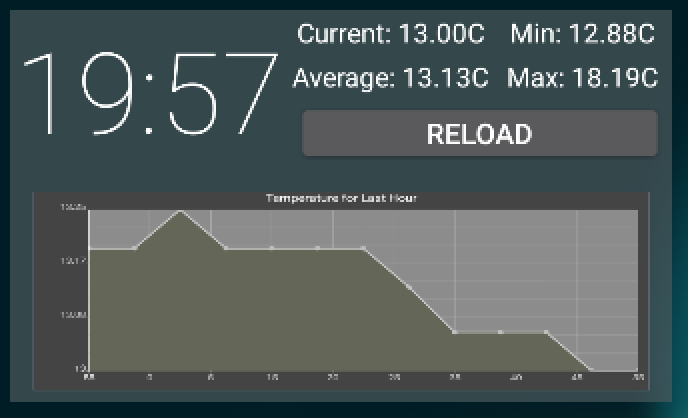
\includegraphics[width=0.5\textwidth]{img/closeup-screenshot.png}
\caption{Close up view of the widget on the home screen.}
\label{fig:closeup}
\end{figure}

My justification for the size of the widget is as follows: I originally chose to use a slim 1 by 4 widget to display all of the data from the server. Widgets cannot be larger than four by default in Android. I chose this width as it maximised the amount of space for my content in the horizontal direction which I feel is more natural for the text content that needs to be displayed. For flair marks I added the graph after the implementation of the main functionality application. I felt natural that this application is extended down by one row. On many Android devices that means that the widget will take up 50\% of the space on a given screen. Looking at other widgets offered on android, this seems to be a common size for widgets such as this. It also has the handy advantage that two independent widgets can be shown on the same screen. 


\section{Implementation}
The code for this widget is actually relatively trivial. There are three major code components of the widget itself with several supporting classes. The most essential class in the project is the \textit{TemperatureDataWidgetProvider}. This class is responsible for the interfaces of every active widget. This class is responsible for firing off an intent to update the widget which is sent periodically. It is also responsible for removing the shared preferences when an app is removed.

The next most important class is the \textit{TemperatureDataWidgetService}. This class implements an \textit{IntentService}. This class is responsible for retrieving the XML data from the remote URL and updating the widget interface with the response. Using an \textit{IntentService} for this prevents interface locking. One service is used for each update requested, so they can effectively run concurrently.

\begin{figure}[ht]
\centering
\subfloat[Widget shown on the home screen]{\label{fig:widget-screen}{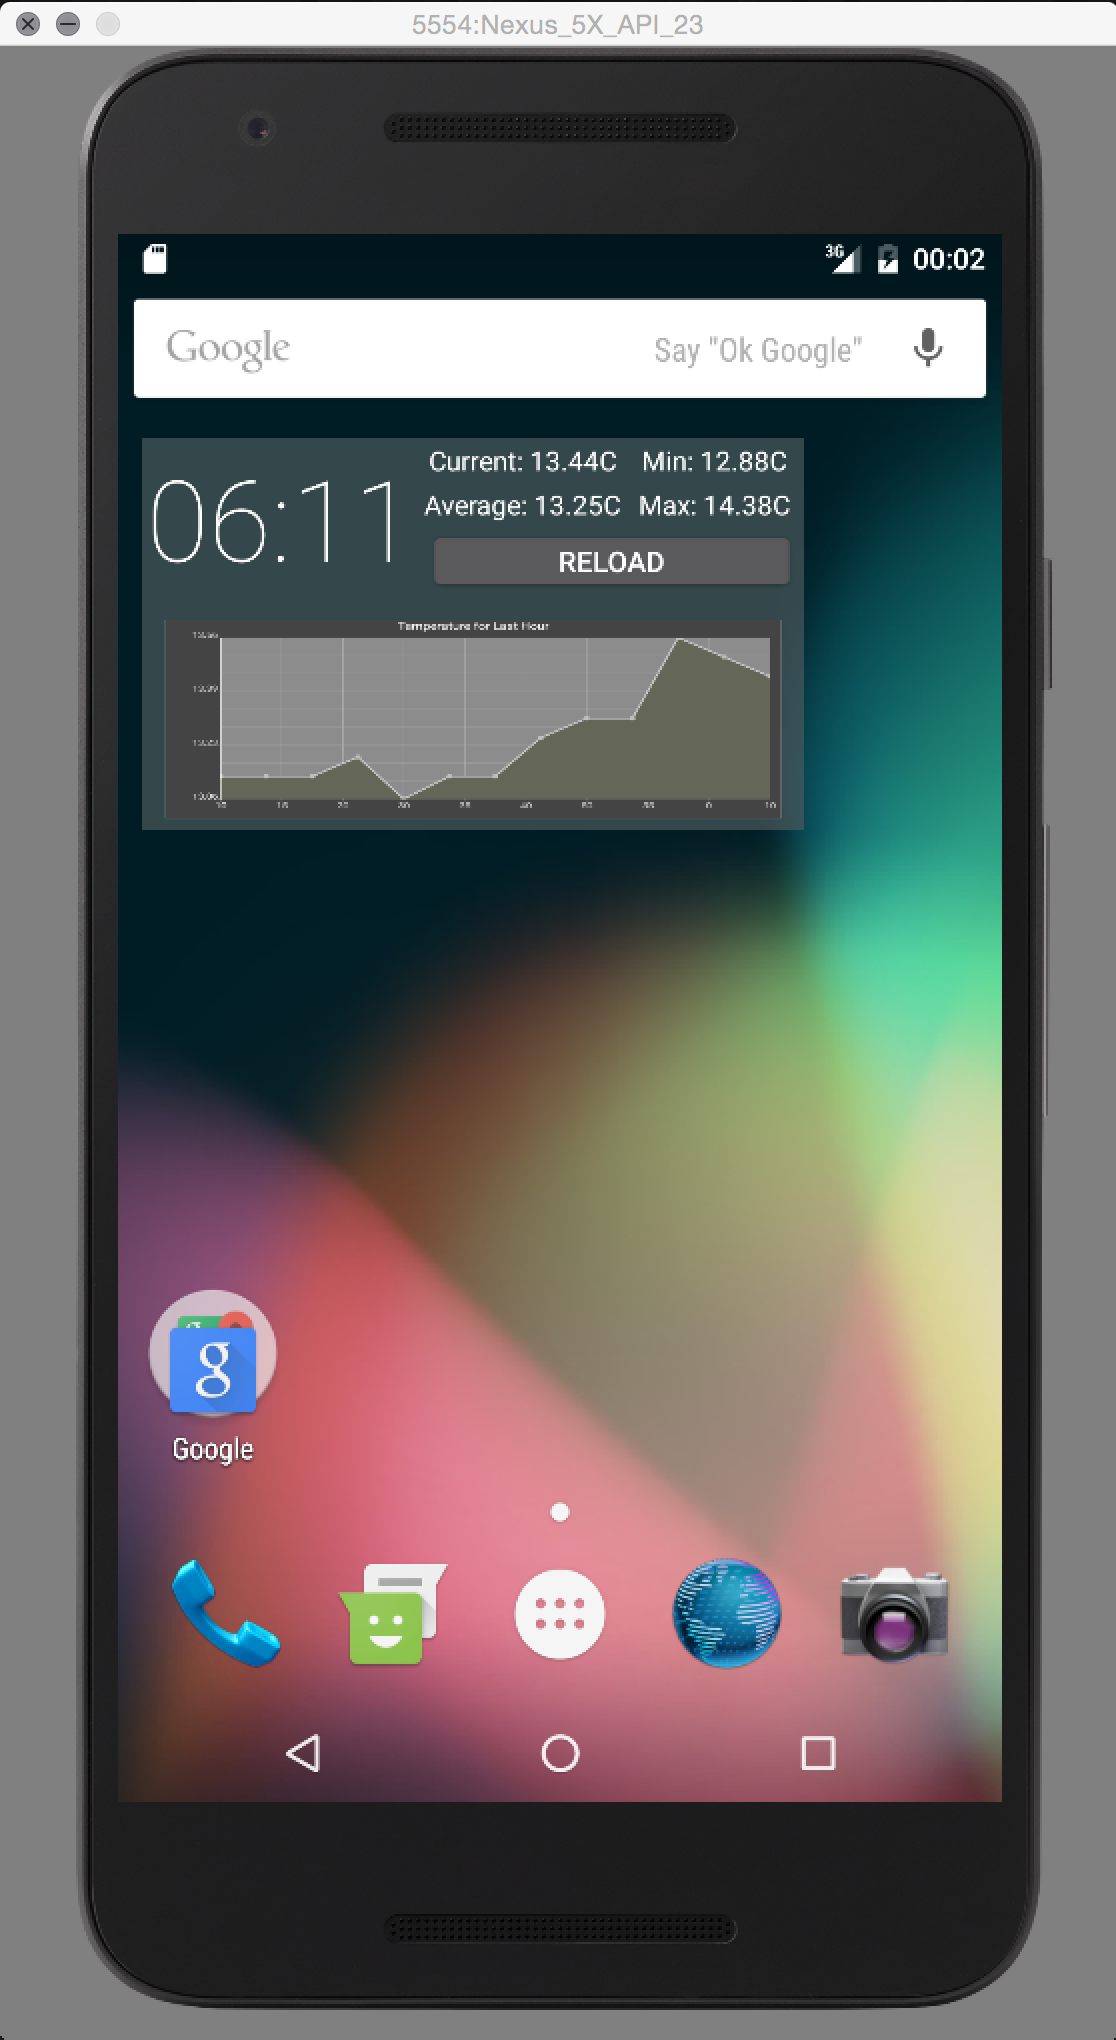
\includegraphics[width=0.3\textwidth]{img/widget-screenshot.png}}}
\subfloat[Widget configuration screen]{\label{fig:config-screen}{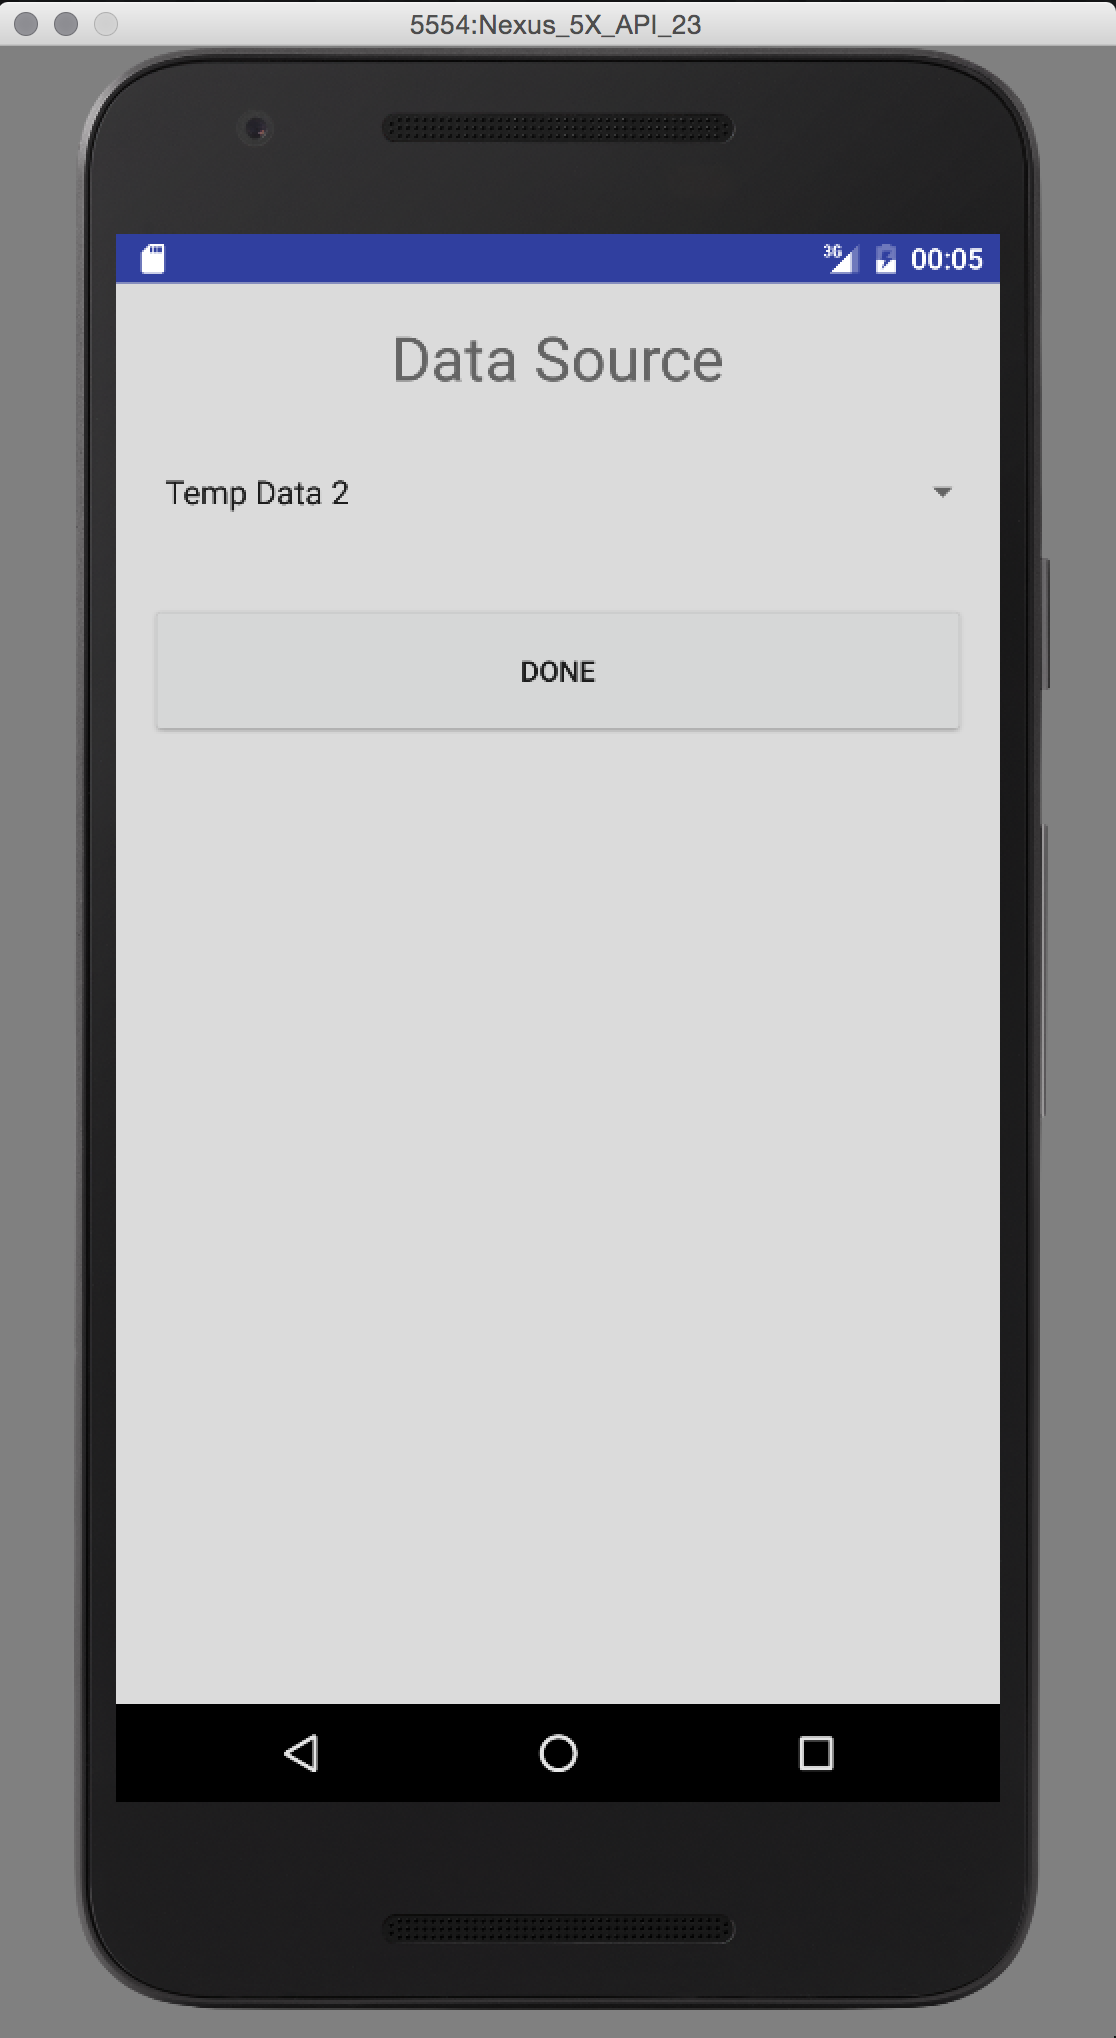
\includegraphics[width=0.3\textwidth]{img/config-screenshot}}}
\caption{The two views of the application}
\label{fig:application-views}
\end{figure}

The third major component is the \textit{TemperatureDataWidgetConfigureActivity}. This class is used to set the shared preferences associated with the widget. There is only one integer shared preference stored in my application. This represents the index of the users choice of data source from the array of data sources provided with the application. This represents an activity that provides UI controls that allow the user to choose their preference of data source.

The other classes in the project are really just helpers for the three main ones. A builder design pattern is used to create a new \textit{RemoteViews} object in order to update the widget interface. This solution was one I settled on after trying several different approaches. The first approach was to use the default method offered by the project scaffold. This uses a static method on the widget provider class to update the UI. I was unhappy with this it seemed like a superfluous use of static methods.

 My initial idea for improvement on this was to have a class which inherits from RemoteViews and implements the desired functionality for building a new UI. I immediately realised that this would not work as the inherited version cannot be displayed by a widget (as noted in the guidelines \cite{android-widget-guidelines}). Subsequently I turned to the builder pattern \cite{vlissides1995design}. 
 
 This pattern is almost overkill for this problem as there are only a limited number of possible combinations of options that could be used. Still, I feel that this is an appropriate solution in this case that ensure that the click handlers are always attached to the interface and allows this code the be reused in multiple parts of the application but with different options (such in with no temperature data in the configuration activity.
 
I chose to implement a \textit{IntentService} to handle retrieving data from a remote server. This is necessary because in order to prevent the GUI locking when performing a potentially long running task (as is the case for networking). There are two obvious choices running a task on another thread in Android. The first is to use a service and the second is to use an \textit{AsyncTask}. Google's indication is that an \textit{AsyncTask} should be use for (relatively) short lived jobs which a service should be used for longer running jobs. 

I used an \textit{IntentService} for two reasons. Firstly I felt that it might be possible on a very slow mobile connection that the job might take a fairly long while. There is also the possibility that the remote URL timeout which would extend the life of the job. Secondly, I wanted to experiment with implementing a service class for my own experience. This also gave me another excuse to play around further with using intents to pass data between the UI and the service.

The remaining classes in the project are those associated with retrieving and processing the response from the remote URL and some data model objects which are created in the parsing process. The whole parsing process returns a single \textit{TemperatureDataObject} which contains a structured representation of the data returned from the URL. This object has various methods associated with calculating the qualities to be displayed by the UI. 

In an attempt to gain some of the flair marks for this assignment I have added an additional feature on my UI in the form of a line graph which shows the temperature readings loaded from the server for the past hour. This is implemented using the AndroidPlot library \cite{android-plot}. Because Android widgets only allow a limited set of interfaces components to be used on the UI a graph object is generated using the data loaded from the server and converted to a Bitmap. This bitmap is then displayed as the contents of an image view (which is a component that is allowed to be used in widgets). 

I encountered several problems when implementing this project. One major problem I encountered was trying to get multiple versions of the widget working independently of one another. The issue I faced was that pressing the reload button on one widget would update the other widget but not itself. I found that this issue was caused by intents passing around the incorrect widget ID and not setting a valid URI.

Another issues which I ran into while developing this application was when refactoring my code I lost the ability to perform click events on the widget. After a bit of debugging I realised that this was due to the event handlers being lost when a new \textit{RemoteViews} object is created which overwrites the previous object.

The work in this project could naturally be extended further with more development time. Support for multiple languages would be a nice addition to the application. Another idea would be to let the user add their own data sources which are stored with the application. This could be easily integrated into the configuration activity. Yet another idea might be to provide support for converting between different types of temperature units (e.g. Fahrenheit, Kelvin).

\section{Self Evaluation}
Based on the work carried out in this assignment, I would award myself an A grade from the guidelines in the student handbook. I feel that I have made a good effort at this assignment. I believe that the application follows the Android widget guidelines fairly closely. I feel that the application provides all of the functionality requested by the brief and implements some additional features in terms of the graph. Based on this I would argue that the grade I have awarded myself is justified.

\clearpage

\begin{landscape}
\section{Test Table}

\begin{longtable}{|l|p{2cm}|p{5cm}|p{7cm}|l|p{3cm}|p{1.5cm}|}
\hline
\textbf{\#} & \textbf{Functional Requirement} & \textbf{Test Description}                                & \textbf{Expected Outcome}                                                                                                                        & \textbf{Pass/Fail} & \textbf{Actual Outcome} & \textbf{Solution} \\ \hline \hline \endhead
1           & FR1, FR3                        & Create the widget                                        & The configuration view is shown. A new widget is added to the home screen after the user closes the configuration.                               & Pass               & As expected.            & N/a               \\ \hline
2           & FR1, FR3                        & Remove the widget                                        & Dragging the widget off the home screen deletes the application without error.                                                                   & Pass               & As expected.            & N/a               \\ \hline
3           & FR1, FR2                        & Reloading the widget                                     & Clicking the reload button should cause the interface to update.                                                                                 & Pass               & As expected.            & N/a               \\ \hline
4           & FR1, FR2, FR3                   & Change the data source used                              & The data source used should be switched by tapping the widget. Checking the log should show that the correct data source is used when reloading. & Pass               & As expected.            & N/a               \\ \hline
5           & FR1, FR2                        & Loading from a broken data source                        & Switching to using the "broken" data source value should a toast indicating that the data cannot be loaded. This also simulates turning off wifi & Pass               & As expected.            & N/a               \\ \hline
6           & FR2                             & Check that the widget is updated every 30 minutes        & After waiting 30 minutes the application should update the interface with new data.                                                              & Pass               & As expected.            & N/a               \\ \hline
7           & FR1, FR2, FR3                   & Create two widgets with different data sources           & The two widgets should work independently and should contain different data.                                                                     & Pass               & As expected.            & N/a               \\ \hline
8           & FR1, FR2                        & With two widgets, reload one.                            & The two widgets should work independently. Reloading one should not effect the other.                                                            & Pass               & As expected.            & N/a               \\ \hline
9           & FR1, FR2                        & With two widgets, change the data source used and reload & The two widgets should work independently. Reloading one should not effect the other.                                                            & Pass               & As expected.            & N/a               \\ \hline
10          & FR1, FR2, FR3                   & With two widgets, delete one.                            & The remaining widget should continue to work and should not be effected                                                                          & Pass               & As expected.            & N/a               \\ \hline

                                                                                                                                                                                                         
\end{longtable}


\end{landscape}

\clearpage
\bibliographystyle{unsrtnat}
\bibliography{references}
\end{document}
